% Created 2017-09-11 seg 08:22
% Intended LaTeX compiler: pdflatex
\documentclass{report}
               \pagestyle{fancy}
\usepackage[latin1]{inputenc}
\usepackage[T1]{fontenc}
\usepackage{graphicx}
\usepackage{grffile}
\usepackage{longtable}
\usepackage{wrapfig}
\usepackage{rotating}
\usepackage[normalem]{ulem}
\usepackage{amsmath}
\usepackage{textcomp}
\usepackage{amssymb}
\usepackage{capt-of}
\usepackage{hyperref}
\usepackage{paralist}
\usepackage{tcolorbox}
\usepackage[table]{xcolor}
\usepackage{lipsum}
\usepackage{caption}
\usepackage{tabu}
\usepackage[subpreambles=true]{standalone}
\usepackage{import}
\usepackage{setspace}
\usepackage{graphics}
\usepackage[linktocpage=true]{hyperref}
\usepackage{tocloft}
\usepackage{minitoc}
\usepackage[portuguese, english]{babel}
\usepackage{subfig}
\usepackage[utf8]{inputenc}
\date{}
\title{}
\hypersetup{
 pdfauthor={},
 pdftitle={},
 pdfkeywords={},
 pdfsubject={},
 pdfcreator={Emacs 25.2.1 (Org mode 9.0.9)}, 
 pdflang={English}}
\begin{document}

\thispagestyle{firstpagestyle}

\import{latex/}{side_info}

\pagestyle{plain}
  \begin{tcolorbox}[colbak=red!5!white, colframe=red!0!white]
  \large{
  \textbf{Highlights}
  \vspace{0.1cm}
  \it
    \import{latex/}{highlights}
  }
  \end{tcolorbox}
  \vspace{-0.2cm}

\setlength{\parindent}{0cm}
\setlength{\parskip}{0.1cm}

\textbf{Global Markets.} European equities are surging, while the S\&P future
is up by 0.55\%. In the meantime, the Mexican peso is up 0.2\% against
the USD, and the yield of the 10 years Treasury is at
2.09\%. Commodities: Oil is up 0.8\% to USD47.8, steel is climbing 1.5\%
and soy prices is about flat.

\textbf{Local News}. The week starts off with the looming risks around the
\textbf{second charge by Attorney General against President Temer}. On this
front, the Folha de Sao Paulo resonates the impression within the
government that, after the affair concerning the General Attorney and
the JBS plea bargain, the President will need to dispense less of a
political capital to safeguard his position.

In fact, in line with the news along the weekend, the government is
feeling so emboldened that is floating the idea of \textbf{voting a full pension system reform by October}. Today, it was down to the O Valor to
circulate this very same idea. In addition, the article makes the
necessary conjectures over what ought to be approved through a
constitutional amendment and what may be fixed through provisional
measures.

On the fiscal front, we sort of have more of the same. \emph{As per} O
Globo, \textbf{the government continues to struggle with disappointing
revenues}, which are threatening its new primary target for the
year. To be sure, the article brings little novelties and, yet again,
revisits all the well mapped out fiscal risks for the year: Cemig's
asset action, provisional measures not yet approved, and so on.

Finally, over the weekend, the news underscored the possibility of a
\textbf{BNDES' transfer of about R\$180bn} to the Treasury, as opposed to the
R\$100bn previously leaked through the press. Moreover, R\$50bn would be
transfered already this year, which was totally out of the radar
screen. Worth pointing out, however, that nothing looked set on the
stone already, since officials of the BNDES themselves were raising
doubts about the whole transaction.

\textbf{Agenda - Highlights}: \uline{Brazil}: IGP-DI, august and market
readout. \uline{US}: Empty.


\rowcolors{2}{grey!15}{white}
\vspace{-0.5cm}
\begin{center}
\begin{tabular}{rlllll}
\textbf{Time} & \textbf{Country} & \textbf{Indicator} & \textbf{Period} & \textbf{Forecast} & \textbf{Impact}\\
\hline
08:00:00 & BZ & IGP-M 1F @ 0,345 & August & 0,34\% mom & Medium\\
08:00:00 & BZ & IPC-S @ 0,10\% & 1W Sep & 0,10\% mom & Medium\\
\end{tabular}
\end{center}

\textbf{Bottom Line}. Global folly and neutral local news should set the
session for a positive start.

\newpage

\section{Brazilian Bonds}
\label{sec:org5e5b2cb}


\begin{center}
\textbf{NTNF} \\
\vspace{0.1cm}
\import{latex/}{NTN-F}
\end{center}
\vspace{0.5cm}

\begin{center}
\textbf{LTN} \\
 \vspace{0.1cm}
\import{latex/}{LTN}
\vspace{0.5cm}
\end{center}

\begin{center}
   \textbf{NTN-B} \\
\vspace{0.1cm}
       \import{latex/}{NTN-B}
       \vspace{0.1cm}
     \end{center}
     \newpage



\begin{center}
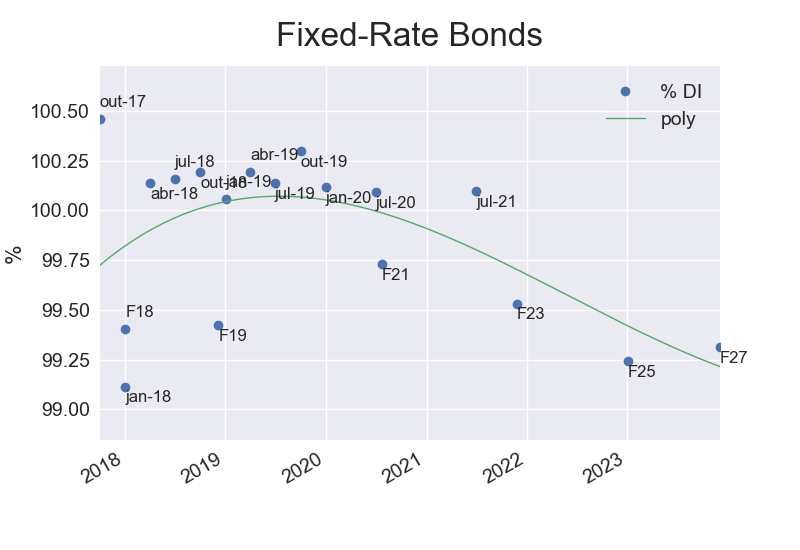
\includegraphics[width=16.0cm]{charts/fixed.png}
\end{center}

\begin{center}
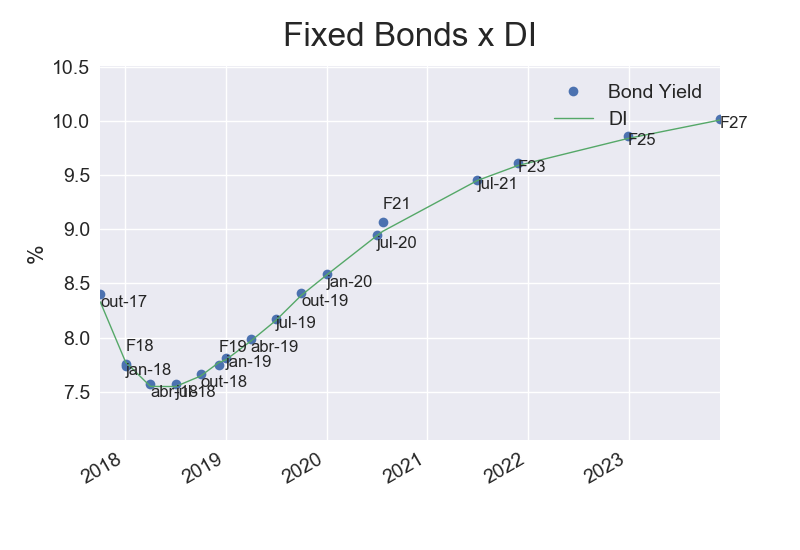
\includegraphics[width=16.0cm]{charts/fixed_di.png}
\end{center}

\begin{center}
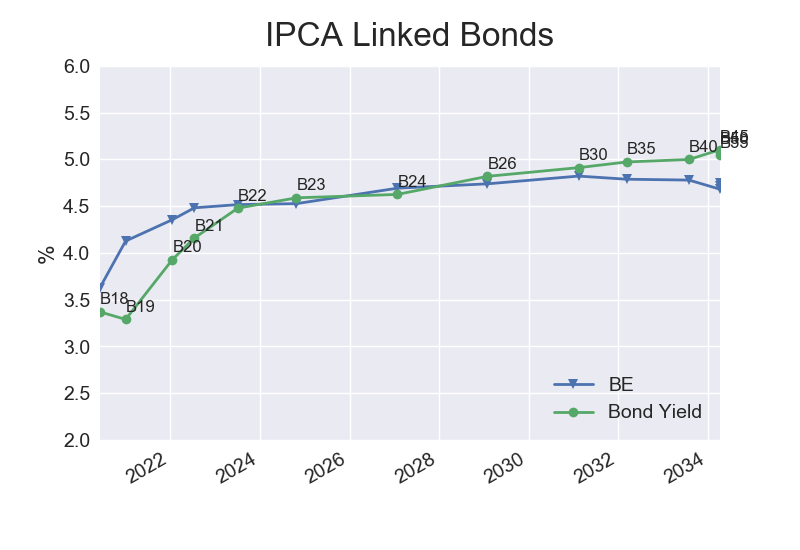
\includegraphics[width=16.0cm]{charts/ntnb.png}
\end{center}


\section{DI - Open Interest}
\label{sec:org71c6115}

  \begin{center}
    \import{latex/}{OpenInterest}
  \end{center}
\newpage

\vspace{3.0cm}
  \begin{center}
    \import{latex/}{DIContracts}
  \end{center}
\newpage


\section{DI - DV01 Table}
\label{sec:orgc699158}

  \begin{center}
    \import{latex/}{DIs}
  \end{center}
\newpage


\section{NTNB FRAs}
\label{sec:org89b3a29}


\begin{center}
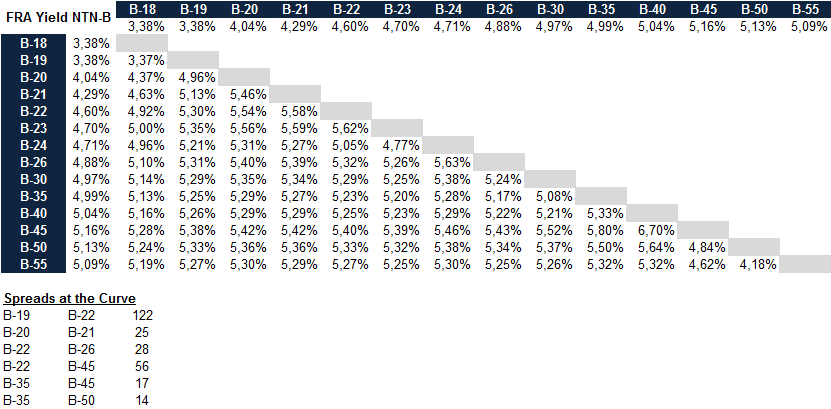
\includegraphics[angle=90,width=10.5cm]{images/FRA_NTNB.png}
\end{center}

\newpage


\section{DI FRAs}
\label{sec:orgf3cc546}
\begin{center}
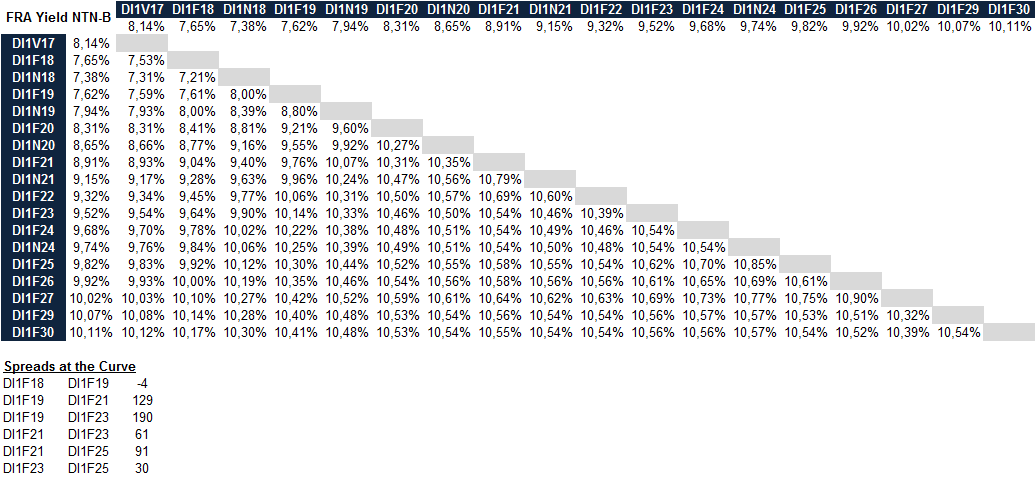
\includegraphics[angle=90,width=10.5cm]{images/FRA_DI.png}
\end{center}

\newpage


\section{Disclaimer}
\label{sec:org7cac1ed}
\smallsize
\begin{quote}
This report has been produced by Guide Investimentos S.A Corretora de
Valores solely for its recipients and should not be distributed
without previous consent from Guide Investimentos S.A.  Although this
report is based upon the most reliable public information, Guide
Investimentos makes no warranties of the reliability of such
information. This document is for informational purposes only and does
not constitute any tender to sell or buy financial
instruments. Information discussed herein is not suitable for all
investors and it does not aim at providing any trading strategy for
individual goals. Investors should have experience and knowledge of
the risks in FX/Fixed Income markets. Guide Investimentos S.A
Corretora de Valores has no obligation to update, revise or modify any
information contained herein. Guide Investimentos and its analysts
shall not be held responsible for any accidental incorrect
information, nor for investment decisions taken based upon the
information contained herein. Additional information discussed on this
report is available upon request.  Analysts each certify that the
views expressed in this report represent only personal views produced
independently, including with respect Guide Investimentos S.A
Corretora de Valores. This report should not be considered as research
report ("relat�rio de an�lise") for the purposes of the article 1 of
CVM Instruction NR 483. Opinions, estimates and projections contained
herein express the current judgment of the analysts build on the date
this report was released and therefore can be changed without
notice. Analysts do not accept any liability that incorrect use of
this report could cause, including financial losses. Upon accepting
this document, one should agree with all the above-mentioned
limitations
\end{quote}
\end{document}
